\chapter{Honeypots}\label{capitulo:honeypots}

% Adaptação livre do texto retirado do endereço \\ \textit{http://www.tracking-hackers.com/papers/honeypots.html}.

O primeiro passo para se entender o que são os \textit{Honeypots}, através de sua definição. Diferente dos \textit{firewalls} ou de Sistemas de Detecção de Intrusão, os \textit{Honeypots} não resolvem um problema em especial. Ao invés disso, são ferramentas altamente flexíveis, com diferentes propósitos, complexidades envolvidas e cujos mecanismos de funcionamento se dão das mais variadas maneiras. Podem realizar atividades que vão desde detectar ataques criptografados à redes \textit{IPv6} até capturar a mais recente fraude financeira envolvendo cartões de crédito. Essa é a flexibilidade que os torna ferramentas tão poderosas. \cite{DefinitioHoneypots}

\textit{Honeypots} são recursos de sistemas de informação, cujos valores residem no acesso não-autorizado ou mesmo o uso ilícito dos mesmos.

Esta definição geral cobre todas as diferentes manifestações de \textit{Honeypots}. Sua natureza é exploratória, baseada em atividades realizadas por indivíduos mal-intencionados, com relação aos sistemas implantados. Conceitualmente, todos os Honeypots trabalham da mesma maneira, não tendo recursos disponíveis publicamente, sendo possível seu acesso, somente através do acesso não-autorizado, realizado através da quebra da segurança envolvida nos sistemas. \cite{WhitepaperHoneypots}

Os \textit{Honeypots} não têm valor real em meio aos ambientes de produção e por isso, não deveriam interagir com nenhuma outra forma de recurso, como outros sistemas ou usuários e, sendo assim, toda e qualquer atividade direcionada aos mesmos deve ser considerada suspeita.

Isso nos remete à situação em que qualquer tipo de interação com os \textit{Honeypots} implantados, pode ser classificada como maliciosa e ilegal, pois toda tentativa de conexão muito provavelmente será relacionada à \textit{scans}, sondagens, ataques ou ao comprometimento do sistema. A abordagem que este tipo de ferramenta toma é realmente simples, no entanto essa é a chave para seu sucesso como grande ferramenta de valor para os profissionais de segurança.

Vantagens: são sistemas conceitualmente simples, o que os torna incrivelmente poderosos.
\begin{itemize}
    \item Pequenos conjuntos de dados, de grande valor: Os \textit{Honeypots} capturam pequenas quantidades de informações. Ao invés de registrar em logs, \textit{Giga-bytes} de dados por dia, em geral, são capturados apenas poucos \textit{Mega-bytes} de dados diários. É comum se encontrar sistemas em produção que geram milhares de alertas por dia, devido à quantidade de acessos que estes têm, provenientes de seus usuários, por estarem realmente expostos e interagindo com uma alta quantidade de outros sistemas. Já os \textit{Honeypots} podem registrar poucas dezenas de alertas por dia, mas que representam muito mais valor que no caso anterior, já que todos estes alertas capturados representam atividades ilegais. Isso facilita o trabalho de interpretação dos dados, tanto em questões de recursos quanto financeiramente, uma vez que o universo de informações a serem analisadas é significantemente menor quando comparado àquele gerado por um sistema real, que se encontra em plena produção.

    \item Novas ferramentas e táticas: Os \textit{Honeypots} são projetados para capturar toda e qualquer informação relacionada às atividades que envolvam interação com o mesmo, podendo revelar novas ferramentas e táticas empregadas pelos atacantes em suas investidas.

    \item Encriptação e \textit{IPv6}\sigla{IPv6}{Internet Protocol Version 6}: Diferente de outras tecnologias, tais como Sistemas de Detecção de Intrusão, pois trabalham bem em ambientes criptografados ou \textit{IPv6}. Não importa o que seja lançado sobre os \textit{Honeypots}, eles irão detectar e capturar tais informações.

    \item Informação: \textit{Honeypots} coletam todas as informações que chegam até eles e poucas ferramentas podem registrar com tanta eficácia este tipo de captura, assim como os \textit{Honeypots} fazem.

    \item Simplicidade: São conceitualmente simples. Não existem algorítmos complexos tanto no processo de desenvolvimento quanto no processo de implantação, não há a necessidade de se manter tabelas de estados ou assinaturas que devam ser atualizadas periodicamente. Quanto mais simples forem as tecnologias envolvidas, menos suscetíveis a falhas ou má-configurações, estas serão.
\end{itemize}

Desvantagens: Assim como qualquer tecnologia, os \textit{Honeypots} possuem seus pontos fracos. Isso porque eles não substituem as tecnologias atuais, mas trabalham em conjunto com as mesmas.
\begin{itemize}
    \item Visão limitada: Os \textit{Honeypots} podem rastrear e capturar atividades que interagem diretamente com eles e por isso, não irão capturar ataques direcionados a outros sistemas, a menos que, o atacante ou a ameaça, interaja também, de alguma maneira, com os \textit{Honeypots}.
    \item Risco: Todas as tecnologias de segurança envolvem riscos. Assim como \textit{firewalls} possuem o risco de serem penetrados, mecanismos de encriptação correm o risco de serem quebrados e Sistemas de Detecção de Intrusão podem falhar na detecção de ataques, os \textit{Honeypots} não são infalíveis. Especificamente, os \textit{Honeypots} estão propensos a serem tomados por atacantes que obtenham sucesso ao se penetrar nos sistemas hospedeiros, por eventuais falhas de configuração ou por conseguirem escalar de maneira adequada seus privilégios. Dependendo do tipo de \textit{Honeypot} implantado, este pode oferecer tanto quanto, ou até menos risco, que um Sistema de Detecção de Intrusão falho, enquanto que existem determinados tipos de \textit{Honeypots} que oferecem riscos reais às redes, uma vez que sejam comprometidos.
\end{itemize}




\section{Classificação dos Honeypots}

Os \textit{Honeypots} são classificados de acordo com seus objetivos e o grau de interação que oferecem aos atacantes. Quanto aos objetivos, existem \textit{Honeypots} de Produção e \textit{Honeypots} de Pesquisa, onde o primeiro é utilizado para mitigar riscos nas redes ativas de organizações e o segundo é empregado na descoberta de novas estratégias de ataque e exploração de falhas de segurança. \cite{HoneynetsEducationalResource}

Quanto ao grau de interação oferecido aos atacantes, temos \textit{Honeypots} de baixa-interação e de alta-interação, onde o primeiro oferece níveis mínimos de interatividade com seus atacantes, na maioria das vezes, emulando Sistemas Operacionais e serviços comprometidos, ao passo que o segundo é composto por um sistema operacional real, onde são introduzidas falhas reais e uma vez no controle de uma máquina comprometida, o atacante pode executar qualquer ação, como em um servidor qualquer, que por ventura tenha sido tomado. \cite{TrappingTheHackers}

A tabela \ref{tabela:honeypots_tipo_interacao} mostra um comparativo de custo de implantação, entre as tecnologias em \textit{Honeypots}, de acordo com seu tipo e nível de interação:

\begin{table}[H]
    \begin{center}
        \caption{\label{tabela:honeypots_tipo_interacao}Tecnologias em \textit{Honeypots} comparadas por Custo de implantação}
        \begin{tabular}{c|c|c}
            \hline
            \hline
                \textbf{Tipo de \textit{Honeypot}} & \textbf{Nível de interação} & \textbf{Custo de implantação}\\
            \hline
                Pesquisa & Baixo & Baixo\\
            \hline
                Pesquisa & Alto & Alto\\
            \hline
                Produção & Baixo & Baixo\\
            \hline
                Produção & Alto & Alto\\
            \hline
            \hline
        \end{tabular}
    \end{center}
\end{table}


\subsection{Honeypots de Produção}

O principal intuito dos \textit{Honeypots} de Produção é fornecer métricas que possam direcionar, de maneira mais efetiva, os esforços dos responsáveis pela administração de redes, afim de obterem níveis de segurança mais finos. Esse tipo de trabalho, é realizado através da coleta e análise dos dados de utilização, provenientes dos serviços oferecidos pelos \textit{Honeypots} de produção. São relativamente fáceis de se utilizar e podem operar camuflados junto à topologia-padrão de rede implantada em uma organização.

Em geral, os principais dados capturados com este tipo de \textit{Honeypot} são pertinentes aos tipos de ataques mais recorrentes que a rede em questão sofre, qual é a localização geográfica dos atacantes e quais são os meios utilizados para tal.

Pode-se utilizar esse tipo de \textit{Honeypot} no intuito de se camuflar servidores de produção que têm grande valor nas organizações. Os atacantes têm em sua maioria, o intuito de vasculhar as redes em busca de máquinas que estejam suscetíveis a falhas de segurança conhecidas e, uma vez encontradas, o processo de exploração dessas falhas permite que seu controle seja tomado sob circunstâncias de sucesso. Sendo assim, é comum que se introduza em meio às redes, máquinas contendo falhas propositais, no intuito de distrair os atacantes. Uma vez identificadas, os esforços para a tomada do controle será quase que unicamente direcionado às mesmas, resguardando as demais de possíveis tentativas de corrupção.

Mesmo que sejam implantados \textit{Honeypots} de baixa interação, os atacantes terão muito tempo investido para que seu sucesso se resuma em pouco resultado, uma vez que o controle pleno de máquinas com esse caráter não é possível. Caso seja escolhida a implantação de um \textit{Honeypot} de alta-interação, medidas de contenção devem ser tomadas, como a implantação de um \textit{firewall} que seja capaz de controlar a saída, \textit{outbound}, dos dados, evitando-se assim, que a partir de uma estação tomada, seja lançado, por exemplo, um ataque de \textit{DoS} em alvos de interesse do atacante.

Uma vez identificados padrões de ataques sofridos pela rede, têm-se condições de elaborar planos de ação, visando mitigar os riscos. Estes planos podem envolver desde melhorias nos \textit{firewalls}, políticas de acessos mais elaboradas, até em mudanças na utilização de senhas, por parte dos usuários, afinal, muitas vezes são identificados ataques por dicionário. Pode-se também incrementar a segurança de uma rede vulnerável com a adição de camadas adicionais de acesso a servidores com grande nível de importância nas organizações, atentando-se ao fato de realizar, progressivamente, filtragens nos dados até que estes cheguem em seus destinos.


\subsection{Honeypots de Pesquisa}

Os Honeypots de pesquisa, visam identificar tanto novos ataques automatizados quanto novas práticas de ataque empregadas pela comunidade \textit{hacker}. Não têm o intuito, assim como os \textit{Honeypots} de Produção, de identificar ataques corriqueiros, e sua finalidade é puramente voltada para a identificação de novos formatos em que possam se enquadrar ameaças desconhecidas ou que tenham sofrido alguma forma de mutação.

São muito empregados na busca por fontes de disseminação de \textit{spam}, uma vez que é possível simular diferentes máquinas rodando diversos sistemas operacionais e serviços, sendo assim, pode-se montar uma infra-estrutura virtual para interceptar este tipo de atividade e tráfego. Pode revelar inúmeros hosts infectados por \textit{worms}, que são cada vez mais presentes nos mecanismos de disseminação de \textit{spam}, o que pode ser definitivo, ao se tentar traçar a topologia total deste problema.

\subsection{Honeypots de Baixa-interação}

\textit{Honeypots} de baixa-interação são compostos por softwares que emulam serviços e sistemas operacionais nas máquinas hospedeiras, assim como por exemplo, faz o \textit{Honeyd}. Seu principal intuito é capturar informações dos atacantes, sem que existam grandes margens para que este se torne um intruso de sucesso, ou seja, consiga tomar controle do sistema hospedeiro.

Tal abordagem, é conseguida quando se têm, por exemplo, uma solução \textit{Honeypot} que escuta todas as portas \textit{TCP} e \textit{UDP} por algum tipo de contato externo. Sendo assim, quando existe alguma comunicação, as informações são guardadas, mas sem que exista realmente, um serviço conhecido, como \textit{FTP}\sigla{FTP}{File Transfer Protocol}, \textit{Telnet} ou \textit{SSH}\sigla{SSH}{Secure Shell} na porta requisitada. Quando um serviço é emulado, por exemplo, um servidor de \textit{FTP}, pode inclusive exibir \textit{banners} nas tentativas de \textit{login} e posteriormente, serem capturados tanto o \textit{login} quanto a senha do atacante, assim como qualquer forma de interação que este tenha com o suposto serviço.

Pode-se escolher perfis de atacantes, através de serviços emulados, por exemplo, implantando-se um pseudo-\textit{Webserver}. Desta maneira, os ataques mais frequentes capturados, serão aqueles destinados a explorar falhas pertinentes ao daemon escolhido. Assim, cria-se um público-alvo específico de estudo.

O filtro pode ocorrer também, com relação ao Sistema Operacional, uma vez que é possível emular comportamentos mediante a \textit{fingerprints} extraídos por ferramentas de \textit{scan} ativas, como o \textit{Nmap} \cite{Nmap}. Os tempos de resposta variam de acordo com o Sistema Operacional selecionado e para que a situação seja mais próxima da realidade de um servidor passível de ataque, escolhe-se serviços que funcionem bem com o ambiente que se deseja emular: um \textit{Webserver} típico em ambientes de produção seria por exemplo, dotado de um \textit{Kernel} do \textit{Linux 2.6.x} e que tenha como \textit{daemon} para servir páginas \textit{Web}, o \textit{Apache 2.2.x} \cite{Apache2}. Dessa maneira é possível restringir cada vez mais o perfil de possíveis atacantes e se estudar as técnicas utilizadas em suas investidas. O tempo de resposta pode ser manipulado maliciosamente pelo \textit{Honeypot} em questão, no intuito de enganar \textit{fingerprints} ativos de Sistemas Operacionais, através de técnicas de emulação que trabalham como implementações específicas da Pilha \textit{TCP/IP}, presentes nos referidos sistemas.

O nível de sofisticação envolvido nas respostas está intrinsicamente relacionado ao tipo de \textit{Honeypot} que se utiliza e podem variar de entre os ambientes escolhidos, oferecendo taxas maiores ou menores de falsos-positivos para os atacantes.

\subsection{Honeypots de Alta-interação}

As \textit{Honeynets} são o exemplo principal de \textit{Honeypots} de alta-interação. Não são compostas por um produto em especial, tampouco por um software específico. Tratam-se de uma arquitetura especial, uma rede inteira de computadores especialmente projetados para sofrerem ataques. A ideia é que se tenha uma arquitetura que crie uma rede altamente controlável, onde todas as atividades sejam monitoradas. Nesta rede, são postas as vítimas propositais: computadores reais, rodando Sistemas Operacionais e aplicações reais.

Os atacantes encontram estas máquinas, lançam esforços para tomá-las e com sucesso, conseguem devido sua iniciativa. Quando se tornam instrusos, não imaginam estar sendo monitorados, por estarem em meio a uma \textit{Honeynet}. Toda a atividade, desde sessões \textit{SSH} encriptadas, \textit{E-Mails} trocados/violados e uploads de arquivos, são capturados sem seu conscentimento.

Isso é possível através da inserção de módulos do \textit{Kernel}, nos sistemas vulneráveis, que capturam as ações tomadas pelos intrusos. Ao mesmo tempo, a \textit{Honeynet} controla as atividades dos atacantes, sendo essa tarefa realizada pelo \textit{gateway Honeywall}, que permite tráfego de entrada, \textit{inbound}, para os sistemas-vítimas e ao mesmo tempo controla todo o tráfego de saída, \textit{outbound}, usando tecnologias de prevenção de intrusão, tais como quando se emprega o serviço \textit{Hogwash} \cite{Hogwash}. Isso permite ao atacante que tenha total flexibilidade ao interagir com o sistema comprometido, ao passo que está limitado no sentido de não conseguir ameaçar diretamente outros computadores que não façam parte da \textit{Honeynet}.


\section{Boas práticas}

Lidando com servidores, a implantação de processos não pode ser levada como uma tarefa banal, assim como é comumente feito em um ambiente de desenvolvimento. Se o objetivo for implantar \textit{Honeypots}, em meio ao ambiente de produção, é importante que seja levada em consideração a segurança do sistema hospedeiro, por isso, existem práticas envolvidas no processo de \textit{deploy} que o tornam mais seguro e consequentemente, menos suscetível a falhas.

Como uma das características principais de um \textit{Honeypot} é atrair a atenção de atacantes em potencial, uma vez que este seja alvo de uma investida de sucesso, pode-se tomar o controle do sistema hospedeiro, caso se trate de um \textit{Honeypot} de alta-interação. Para evitar que este mesmo sistema não seja utilizado para comprometer mais computadores, ou mesmo para disseminar atividades ilegais, deve-se apertar a segurança tanto quanto seja possível, e uma das maneiras mais eficientes consiste em limitar o escopo dos serviços, ou aplicações, que são postos em execução. Isso é possível graças à uma ferramenta desenvolvida por \textit{Niels Provos}, um dos grandes estudiosos no ramo de segurança de redes e \textit{Honeypots}. Uma breve visão sobre sua utilização será exposta e como fator opcional para o aumento da segurança em testes coleta de informações, utilizando-se \textit{Honeypots}, recomenda-se que os ambientes sejam preparados com base neste utilitário chamado \textit{Systrace}.

\subsection{Protegendo serviços}

Trata-se de uma ferramenta que força políticas de segurança relacionadas às chamadas de sistema\cite{Systrace}. Isso faz com que um programa tenha seu acesso limitado, de acordo com o tipo de ação que pretende realizar no sistema. As operações não autorizadas disparam alarmes, permitindo ao usuário refinar a política de segurança implantada.

Ao lidar com aplicações complexas, é árdua a tarefa de se definir todas as chamadas de sistema que podem ser autorizadas. É impraticável o ato de prever todos os seus ciclos de execução, aliados aos privilégios requeridos em cada instante. Para isso, o \textit{Systrace} \cite{SiteSystrace} realiza o monitoramento do executável, notificando o usuário sobre cada chamada de sistema cujos privilégios necessários sejam superiores aos que foram concedidos inicialmente. Depois de ser recebida a avaliação, é criada uma regra que será englobada, posteriormente, à sua política de segurança. No entanto, devido ao comportamento observado não ser totalmente previsível, é comum que esporadicamente sejam disparados alertas de segurança relacionados às chamadas de sistema, sendo que com o tempo, a tendência de uso determina que estes alertas se tornem cada vez mais raros, até que a política de segurança seja refinada o suficiente, de modo que, durante a execução do binário monitorado não sejam gerados mais alarmes durante todo o seu ciclo de vida.

As políticas de segurança podem ser aprendidas automaticamente, sendo estas aplicáveis a ambientes de testes, sem a necessidade mandatória de interferência ou pós-processamento manual. É desejável que se construa ambientes seguros em servidores, por exemplo, onde um serviço possa rodar isolado das demais, garantindo que qualquer comportamento anormal só afete a ele mesmo, não interferindo no sistema como um todo. Isso é obtido, empregando-se varias técnicas de \textit{sandboxing}, e o \textit{Systrace} pode ser utilizado como peça fundamental no processo de obtenção de um ambiente próximo do idealizado.

O encapsulamento de binários em ambientes \textit{sandbox}, torna-se extremamente útil quando se deve lidar com exemplares cujo código-fonte não é disponibilizado, ou mesmo quando tratam-se de fragmentos advindos de grandes projetos de código-fonte aberto e que, devido sua grande extensão e complexidade, não têm todo o seu comportamento devidamente assegurado por técnicas que envolvam suites de testes unitários e cobertura de código efetivamente implantadas. As motivações para a utilização do \textit{Systrace} extendem-se também aos casos onde é imprescindível a realização de auditorias nos sistemas, seja por fins de pesquisa ou pelo fato de que sua execução pode ser classificada como parte de um conjunto de ações críticas, perante o Sistema Operacional e à estrutura dependente deste, como serviços em execução e informações sensíveis hospedadas.

As chamadas de sistemas podem ser re-escritas dinamicamente, provendo ao Sistema Operacional, um caráter semelhante ao encontrado em ambientes chroot virtuais, além de previnir race conditions na interpretação dos argumentos passados\cite{RACEARGS}.

É possível monitorar máquinas remotas e gerar alertas em uma central, indicando operações que a política de segurança existentes não cobrem. Sendo assim, pode-se detectar intrusões e também realizar a prevenção das mesmas, mitigando riscos potenciais, em ambientes de produção, através de um processo contínuo de monitoramento e correções.

Aplicações ordinárias podem necessitar de privilégios maiores com relação aos que se deseja conceder. O \textit{Systrace} pode interferir no modo em que executam, permitindo delimitar pontos onde os privilégios sejam concedidos, sem que seu comportamento seja alterado. De um modo geral, os privilégios são escalados somente no instante em que as chamadas de sistema associadas necessitam, desde que sejam denominadas confiáveis. Isso elimina a necessidade de se ter ciclos completos de execução marcados como privilegiados, por exemplo: através do uso das \textit{flags} \textit{setuid} e \textit{setgid} (que poderão ser removidas completamente dos binários em questão) ou com a utilização de usuários privilegiados no sistema destinados exclusivamente para a execução de aplicações específicas.


\section{Organizações envolvidas}

A comunidade conta com várias organizações, responsáveis pelo desenvolvimento das tecnologias em \textit{Honeypots} e identificação de ameaças e tendências de ataques globais. Para tal, as organizações contam com o apoio de instituições parceiras, que em geral compõe-se principalmente por Universidades e Empresas que reconhecem a importância deste tipo de trabalho.

São apresentadas a seguir, algumas das organizações mais influentes so setor mundial, no que compete à pesquisa e desenvolvimento de tecnologias em \textit{Honeypots}. Existe também, a preocupação em apresentar duas iniciativas nacionais relacionadas, que também exercem um papel extremamente importante perante à comunidade mundial e são ótimos pontos de partida para organizações estabelecidas em território brasileiro e que se interessam em estabelecer parceirias no combate às atividades ilegais, realizadas na \textit{Internet}.


\subsection{Honeynet Project}

% Adaptação livre do texto retirado do endereço \textit{http://www.honeynet.org/about}.

Fundada em 1999, o \textit{Honeypot Project} é uma organização internacional, de pesquisa, dedicada à melhoria da segurança da \textit{Internet}, sem custo algum para o público. Seus voluntários estão engajados com o movimento \textit{Open Source} e visam trazer valor à comunidade por meio de medidas como o alerta sobre ameaças e vulnerabilidades presentes na \textit{Internet} atualmente.

Muitas organizações e indivíduos não sabem que são alvos de ataques, tão pouco sabem quem os ataca, quais são seus motivos e como isso é realizado. Provendo este tipo de informação, é possível que se entenda essa dinâmica e então sejam tomadas medidas para que as ameaças sejam mitigadas. Essas informações são disponibilizadas através de uma série de \textit{whitepapers} chamados \textit{Know your Enemy}. \cite{KnowYourEnemy} \cite{KnowYourEnemy2}

São compartilhados, com os especialistas em segurança, dados que ajudam no processo de defesa de seus recursos. Historicamente, as informações sobre atacantes eram limitadas às ferramentas utilizadas pelos mesmos. Como diferencial, são oferecidos também os motivos de ataque, a maneira como se comunicam, as datas de ataques e as ações tomadas quando os sistemas são comprometidos. Além da série \textit{Know your Enemy}, existem desafios lançados chamados \textit{Scan of the Month}, um agregador em conjunto ao blog oficial \cite{Agregador} e várias ferramentas \cite{FerramentasHoneynet}, responsáveis por muitas dessas informações adicionais.


\subsection{Leurrecom}

% Adaptação livre do texto retirado do endereço \textit{http://www.leurrecom.org/project.php}.

Trata-se de um projeto que visa a implantação de uma plataforma em \textit{Honeypots} distribuída e de larga escala. São instalados sensores em diversas partes do mundo, onde intuito é a geração e análise posterior dos logs de atividades. \cite{Leurre}

Esse arranjo abrange hoje, em torno de 30 países distribuídos pelos 5 continentes, o que fornece uma medida muito próxima da realidade no que tange ao comportamento das atividades ilegais ao redor do globo. Os dados são armazenados em bancos de dados sofisticados, com suporte à \textit{SQL} e acompanham dados enriquecidos de informações contextuais, tais como localização geográfica dos atacantes, \textit{fingerprint} de seus sistemas operacionais e busca reversa por seus endereços de \textit{DNS}.

É oferecida aos seus parceiros, uma interface intuitiva de consulta aos dados, facilitando ainda mais as tarefas gerenciais através da possível elaboração de relatórios de alto-nível. Tais informações podem revelar qual é a frequência com que os ataques são lançados de diversos pontos, podendo ser comparados uns aos outros em termos de ferramentas utilizadas nos ataques, quem são especificamente os atacantes e quais foram as técnicas empregadas pelos mesmos em suas investidas.

Para se tornar parceira, uma instituição precisa somente concordar em hospedar em suas dependências de infra-estrutura, umas das plataformas oferecidas pelo projeto. Como consequência, é concedido o direito de acesso a um banco de dados que fora alimentado durante mais de 3 anos com atividades sendo registradas. É também requerido que se assine um termo de não-revelação pública dos nomes de outros parceiros e das identidades dos atacantes.


\subsection{Honeynet.BR}

% Adaptação livre do texto retirado do endereço \textit{http://www.honeynet.org.br/}.

Devido ao crescente interesse no desenvolvimento de tecnologias em \textit{Honeytraps} por parte da comunidade e dos estudos dirigidos às \textit{Honeynets}, liderados principalmente por \textit{Lance Spitzner}, o grupo brasileiro \textit{Honeynet.BR}, membro da \textit{Honeynet Research Alliance} desde Junho de 2002, investiu esforços na criação de uma solução robusta em \textit{Honeypots}, de modo que fosse efetiva a sua implantação em instituições de pesquisa e que pudesse revelar, em conjunto com muitas outras instituições, o comportamento das ameaças em território nacional.

Os dados são integrados com outras instituições credenciadas internacionalmente e com isso é possível observar as atividades em âmbito global, através de um projeto em comum. Seus idealizadores no Brasil pertencem ao Instituto Nacional de Pesquisas Espaciais (\textit{INPE})\sigla{INPE}{Instituto Nacional de Pesquisas Espaciais}, em conjunto com o \textit{CERT.br} \sigla{CERT}{Computer Emergency Response Team}. \cite{CERTBRHoney}

\subsubsection{Topologia}

A arquitetura da rede \textit{Honeynet.BR} consiste basicamente em uma \textit{Honeynet GenII} com algumas modificações. Sua rede é composta de um segmento de rede administrativo e uma \textit{Honeynet}.

A rede administrativa é composta por três componentes principais: um \textit{Firewall}, um \textit{Sistema de Detecção de Intrusões} e uma máquina para \textit{Computação Forense}.

O \textit{Firewall} consiste em um sistema \textit{OpenBSD} operando em modo \textit{bridge}, rodando \textit{pf} (\textit{OpenBSD Packet Filter}), logando todo o tráfego e limitando a banda de saída.

Um programa foi desenvolvido para limitar a atividade do intruso, interagindo com o \textit{pf} para dinamicamente, mudar as regras de \textit{firewall}. Esse programa, chamado \textit{sessionlimit}, monitora o tráfego de saída, visando detectar e parar atividades maliciosas, tais como \textit{portscans} provenientes da \textit{honeynet}.

O Sistema de Detecção de Intrusão opera com as duas interfaces de rede, uma conectada à rede administrativa e a outra com a honeynet. A última, captura todo o tráfego e não possui endereço de \textit{IP}. Essa máquina gera alertas e envia emails diários com sumários para todos os membros do projeto.

A máquina utilizada para computação forense, é utilizada para armazenar e analizar imagens das partições provenientes das máquinas que pertencem à \textit{honeynet}, além das ferramentas deixadas pelos intrusos.

A figura \ref{figura:topologia_honeynet} mostra esquematicamente, a topologia de rede que abordada.

\begin{figure}[H]
    \begin{center}
        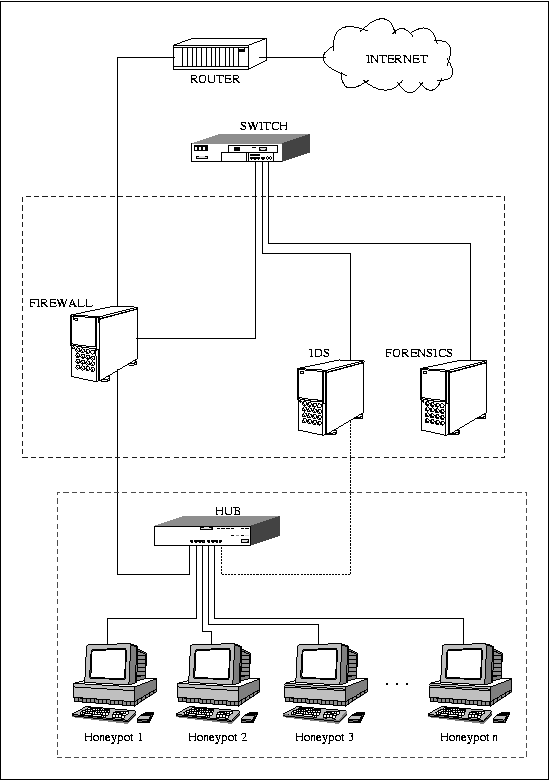
\includegraphics[scale=0.6]{./figuras/topologia-honeynet-br-GS.png}

        \caption{\label{figura:topologia_honeynet}Topologia da \textit{Honeynet}.}
    \end{center}
\end{figure}


\subsubsection{Honeynet}

A \textit{honeynet} é composta por várias máquinas rodando diferentes sistemas operacionais e serviços, são dotadas de utilitários para logar as atividades e o tráfego interno da \textit{honeynet} é capturado pelo Sistema de Detecção de Intrusões.

As honeynets permitem que sejam observadas as ações e técnicas utilizadas pelos atacantes, além de poderem capturar as ferramentas que estão sendo distribuídas pela comunidade blackhat. Em certas ocasiões, é possível também, monitorar eventuais conversas entre os atacantes, que podem guiar a um melhor entendimento sobre as suas motivações e perfis psicológicos.

\subsubsection{Honeytraps}

Os \textit{honeytraps}, são em geral, divididos em duas categorias: passivos e ativos. Os \textit{honeytraps} passivos são sistemas de baixa interatividade, ou seja, permitem somente uma baixa-interatividade e nenhum acesso aos sistemas hospedeiros. Exemplos de honeytraps são os da família \textit{Back Officer}, \textit{Deception Toolkit}, \textit{Scpecter} e \textit{Honeyd}. São extremamente úteis na detecção de tendências de ataques, atividades de \textit{scan} e servem como agentes para o disparo de alertas prematuros ou como sistemas de detecção de atividades não-autorizadas em ambientes de produção.

Os \textit{honeytraps} ativos permitem, em geral, interações completas entre os atacantes e os \textit{hosts}, que podem estar conectados a uma \textit{LAN}, que é o caso das \textit{honeynets}, ou podem ser emulados em um único sistema, com uso de mecanismos de virtualização. No último caso, podem ser utilizadas aplicações como \textit{VMWare}, \textit{UML} (\textit{User-Mode-Linux})\sigla{UML}{User-Mode-Linux} ou \textit{Decoy Server} (formalmente conhecido por \textit{ManTrap}).


\subsection{Project Honey Pot}

% Adaptação livre do texto retirado do endereço \textit{http://www.projecthoneypot.org/about\_us.php}.

O \textit{Project Honey Pot} é o primeiro e o único sistema distribuído para a identificação de \textit{spammers} e os \textit{spambots} que utilizam para obter endereços de \textit{E-Mail} dos \textit{websites}. Integrando-se ao \textit{Project Honey Pot}, pode-se instalar endereços de \textit{E-Mail} com identificadores especiais relacionados ao momento de acesso de cada visitante do site em que foi implantado, o que os relaciona com seu respectivo endereço de \textit{IP}. Se algum destes endereços começar a receber \textit{E-Mails}, não só é gerado um alerta sobre o spam recebido, como também é indicado o momento exato em que o endereço foi capturado e o \textit{IP} referente ao infrator.

Para participarem do \textit{Project Honey Pot}, os webmasters precisam somente instalar o software provido pelo projeto em uma localização escolhida, em seus \textit{websites}. O restante do processo é conduzido pela central responsável pela geração dos \textit{E-Mails} a um baixo custo de banda, não sendo assim, nocivo em termos de geração de tráfego adicional em níveis prejudiciais.

Esses dados gerados pelo \textit{website} são coletados, processados e compartilhados com seus responsáveis. Existem parcerias estabelecidas com promotorias de justiça responsáveis pelo enquadramento das atividades reportadas como sendo ilegais, assim como pela punição dos \textit{spammers} identificados.

Adicionalmente, as mensagens de \textit{E-Mail} geradas pelos spammers são capturadas, analisadas e compartilhadas com desenvolvedores e pesquisadores na área \textit{anti-spam}. Os dados coletados pelo \textit{Project Honey Pot} irão ajudar a construir uma nova geração de ferramentas em software \textit{anti-spam}.

O \textit{Project Honey Pot} foi criado por \textit{Unspam Technologies, Inc}, uma companhia \textit{anti-spam} com a missão singular de ajudar no projeto e aplicação de leis efetivas \textit{anti-spam}.


\subsection{Brazilian Honeypots Alliance}

O objetivo deste projeto é aumentar a capacidade de detecção de incidentes, correlacionar eventos e analisar as tendências no espaço de Internet brasileiro. Para que isso seja possível, o projeto foca em definir uma rede de máquinas comprometidas com \textit{Honeypots} de baixa-interação (\textit{Honeyd}), cobrindo a maioria do espaço de endereços de IPs brasileiros, construir um sistema de análise de dados que permita o estudo das tendências de ataques e suas correlações e trabalhar com os times de Resposta a Incidentes de Segurança de Computadores, para que a informação seja disseminada.

% http://www.honeypots-alliance.org.br/

A figura \ref{figura:distribuicao_honeypots} mostra a distribuição dos \textit{Honeypots} pelo território brasileiro, relacionando as instituições colaboradoras, que são enumeradas:

\begin{figure}[H]
    \begin{center}
        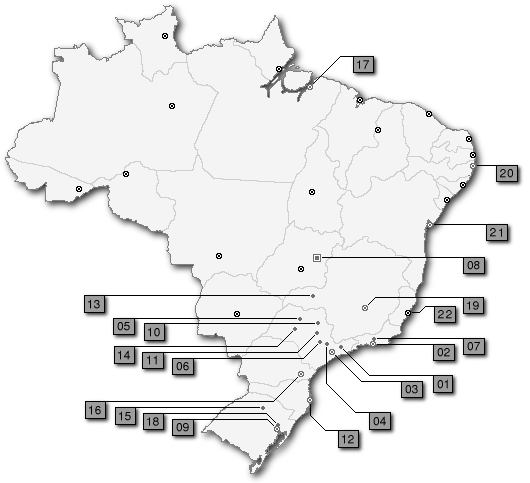
\includegraphics[scale=0.6]{./figuras/honeypots-alliance-map-GS.png}

        \caption{\label{figura:distribuicao_honeypots}Distribuição dos Honeypots pelo território nacional.}
    \end{center}
\end{figure}

A tabela \ref{tabela:instituicoes_honeypots} relaciona as instituições com sua respectiva enumeração, apresentada na figura anterior:

\begin{table}[H]
    \caption{\label{tabela:instituicoes_honeypots}Distribuição de \textit{Honeypots} em instituições brasileiras.}
    \begin{center}
        \begin{tabular}{c|c|p{8cm}}
            \hline
            \hline
                \textbf{\#} & \textbf{Cidade} & \textbf{Instituição}\\
            \hline
                01 & São José dos Campos & INPE, ITA\\
            \hline
                02 & Rio de Janeiro & BNDES, CBPF, Embratel, Fiocruz, Furnas, PUC-RIO, RedeRio\\
            \hline
                03 & São Paulo & ANSP, Banco Real, CERT.br, Diveo, Durand, TIVIT, UNESP, UOL, USP\\
            \hline
                04 & Campinas & CenPRA, ITAL, UNICAMP\\
            \hline
                05 & São José do Rio Preto & UNESP\\
            \hline
                06 & Piracicaba & USP\\
            \hline
                07 & Petrópolis & LNCC\\
            \hline
                08 & Brasília & Banco do Brasil, Brasil Telecom, CTIR Gov, Ministério da Justiça, TCU\\
            \hline
                09 & Porto Alegre & CERT-RS\\
            \hline
                10 & Ribeirão Preto & USP\\
            \hline
                11 & São Carlos & USP\\
            \hline
                12 & Florianópolis & UFSC DAS\\
            \hline
                13 & Uberlândia & CTBC Telecom\\
            \hline
                14 & Lins & FPTE\\
            \hline
                15 & Passo Fundo & UPF\\
            \hline
                16 & Curitiba & Onda, PoP-PR, PUCPR\\
            \hline
                17 & Belém & UFPA\\
            \hline
                18 & São Leopoldo & Unisinos\\
            \hline
                19 & Belo Horizonte & CSIRT PoP-MG, Diveo\\
            \hline
                20 & Recife & EMPREL\\
            \hline
                21 & Salvador & UFBA\\
            \hline
                22 & Vitória & PoP-ES \\
            \hline
            \hline
        \end{tabular}
    \end{center}
\end{table}


\section{Implicações Legais}

% Adaptação livre do texto retirado do endereço \textit{http://www.honeynet.org/node/458}.

Os \textit{Honeypots} foram utilizados peloa comunidade de especialistas em segurança por anos, até a presente dada. Foram aplicados com uma variedade imensa de propósitos e hoje em dia, seu uso comum é a obtenção e análise de informações relacionadas ao comportamento das redes. Desde o princípio de sua utilização, geraram discussões perante a comunidade sobre suas implicações legais. No entanto, ao longo dos anos esse debate aparentemente se extinguiu e a maioria das organizações o consideram como a menor das implicações. \cite{AreHoneypotsIllegal}

A maioria dos produtores de software voltados para segurança, como \textit{Symantec}, \textit{MCaffe}, \textit{Websense} e \textit{Sophs}, assim como muitos \textit{CERTs} de vários países, implantam ativamente esses mecanismos para a melhoria da segurança da Internet. Os \textit{Honeypots} não têm por natureza, incitar a invasão ou práticas ilegais, assim como não força os atacantes a cometerem delitos aos quais não estejam propensos naturalmente. São sistemas sem valor, quando analisados em conjunto aos demais presentes em um ambiente de produção, por isso, teoricamente nunca deveriam interagir com outros sistemas ou usuários. Adicionalmente, estes sistemas, a priori, não possuem contas abertas e por isso, a única maneira de se obter acesso aos mesmos, é quebrando sua segurança.

Uma visão não técnica sobre o assunto, seria descrita facilmente ao se comparar o conceito de invasão em \textit{Honeypots} ao roubo de carros: Suponha que exista um estacionamento de carros, cuja lotação encontra-se em um nível máximo, ou mesmo perto disso, analogamente aos espaços de \textit{IP} preenchidos por vários computadores. Cada qual é provido de trancas funcionais e alguns destes possuem câmeras em seus interiores (acionadas via sensores de movimento), representando os \textit{firewalls} e \textit{Honeypots} respectivamente. Ninguém, além dos legítimos donos dos carros, deveriam obter acesso ao interior dos mesmos, pois estes encontram-se seguros, através de suas trancas, e somente acessos autorizados são aceitos. No entanto, se alguém mal-intencionado decidir praticar um roubo, ou qualquer atividade ilegal, envolvendo o acesso não-autorizado ao interior do veículo, este terá que quebrar a segurança empregada no mesmo, arrombando tais trancas ou utilizando técnicas que não requerem as chaves do seu dono original para isso, como o estilhaçamento de seus vidros. Se efetivada com sucesso, essa invasão ao veículo pode ser monitorada através da câmera instalada. O que se aplica totalmente aos mecanismos de captura de informações presentes nos \textit{Honeypots}. Os dados gerados pelo intruso são armazenados a partir do momento em que este toma o interior do veículo, pois o acionamento se dá pelos sinais enviados pelos sensores.

Tendo em mente o que representam os Honeypots, um consenso que se tem sobre o assunto é que sua implantação é extremamente cabível para as organizações, desde que seus sistemas não sejam tratados com negligência. Deve-se atentar ao fato de que alguns tipos de \textit{Honeypots} podem trazer riscos às redes de computadores, caso não sejam bem configurados e monitorados. Sendo assim, é da responsabilidade de seus administradores, que estes não sejam utilizados como meio de causar danos às demais organizações, pois caso isto aconteça, estarão passíveis de processos judiciais.
